\documentclass{standalone}
\usepackage{tikz}
\usetikzlibrary{patterns, positioning}
\usepackage[sfdefault]{ClearSans} %% option 'sfdefault' activates Clear Sans as the default text font
\usepackage[T1]{fontenc}

\begin{document}
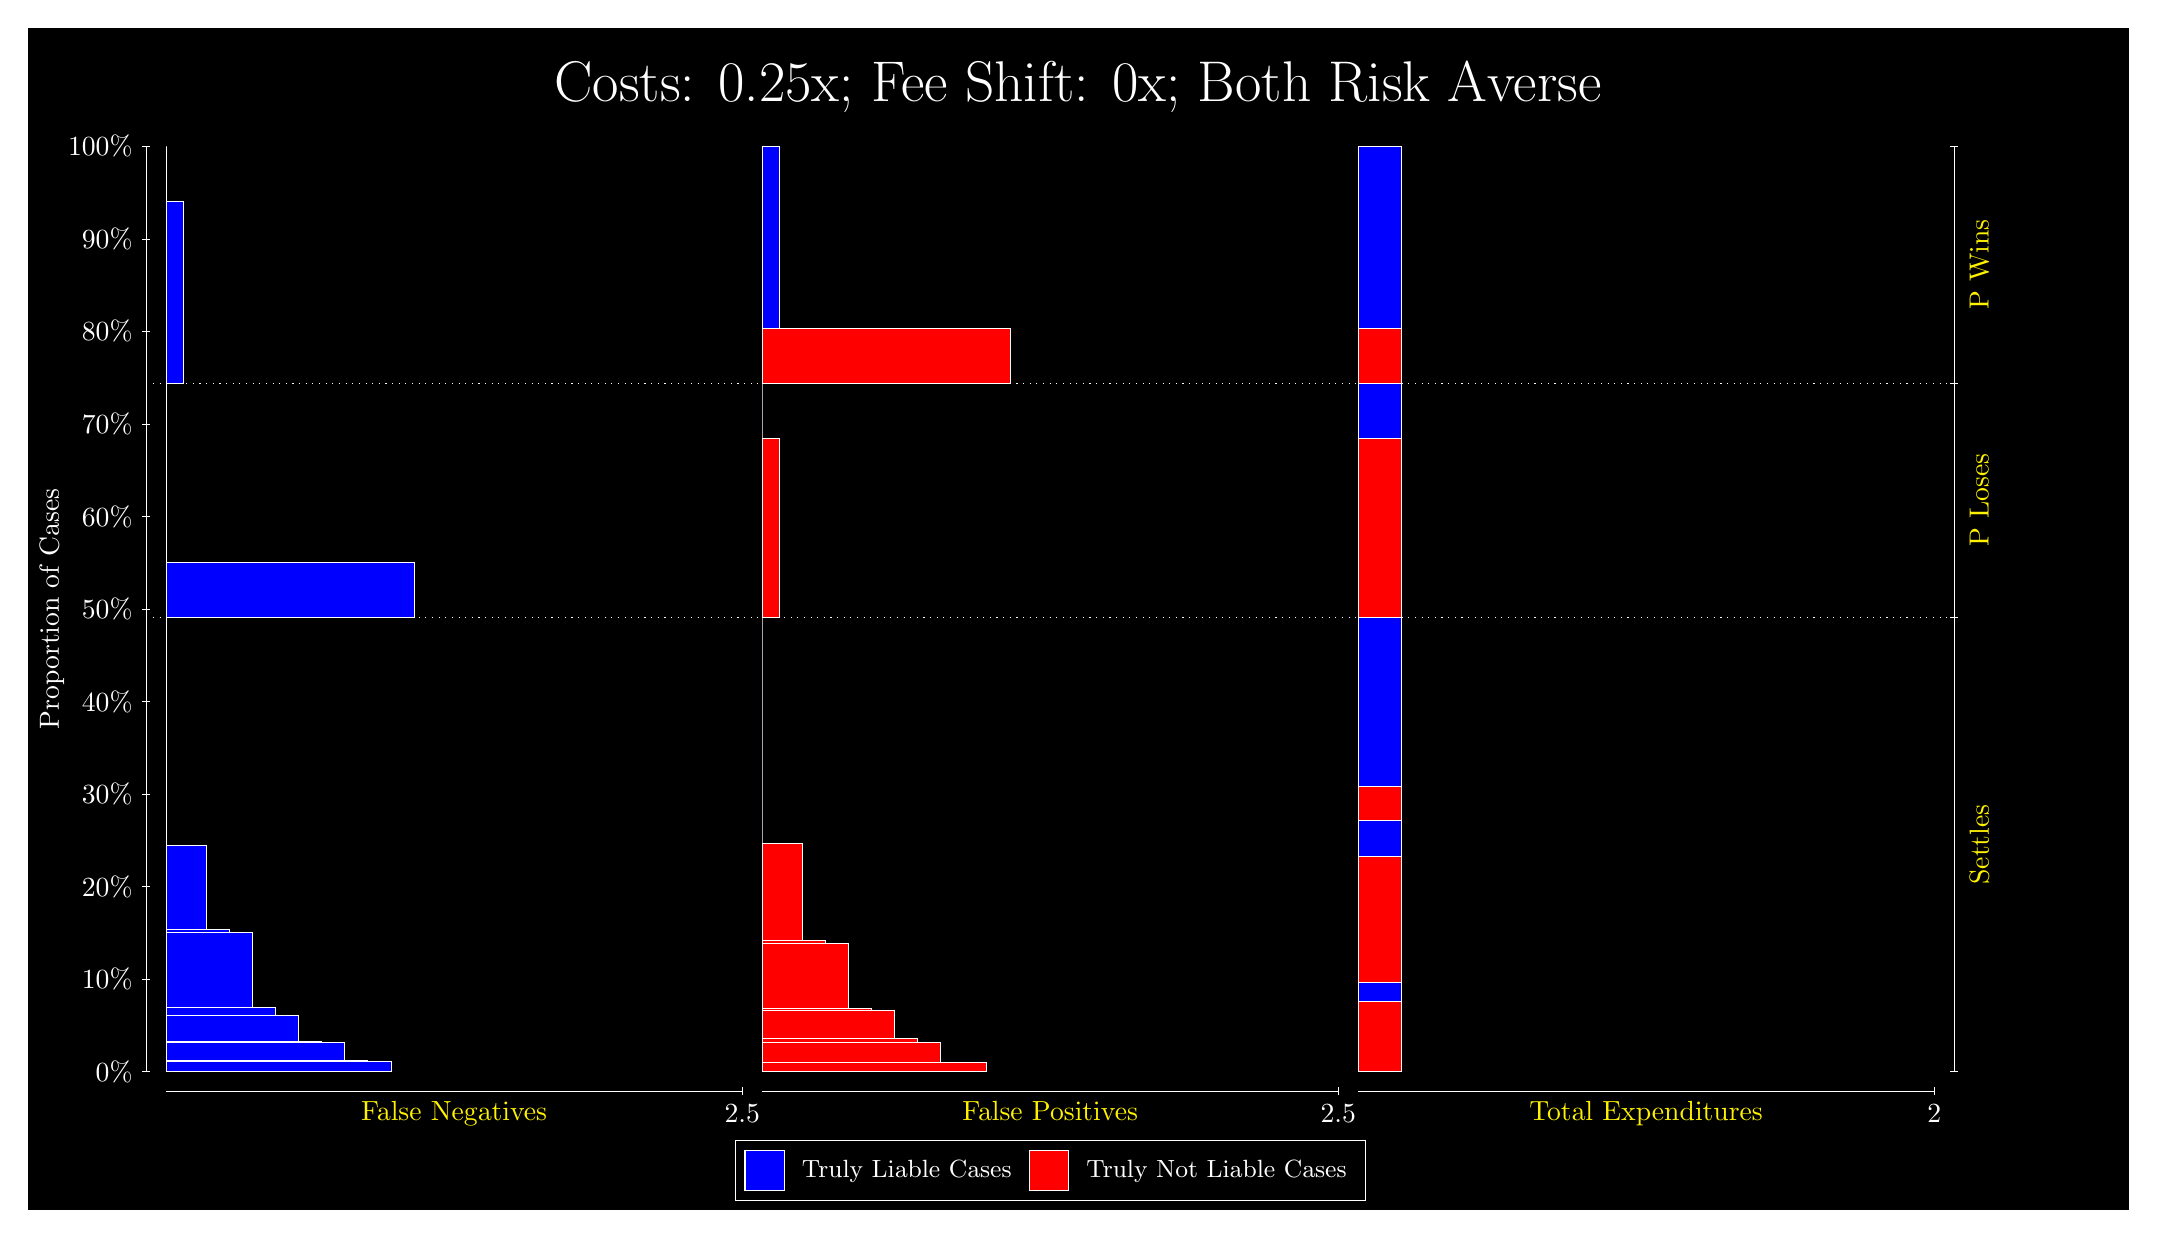
\begin{tikzpicture}
\draw[fill=black] (0,0) rectangle (26.667,15);
\draw[text=white] (0,13.5) rectangle (26.667,15) node[midway] {\huge Costs: 0.25x; Fee Shift: 0x; Both Risk Averse};
\draw[white, very thin] (1.5,1.75) -- (1.5,13.5);
\node[rotate=90, text=white, anchor=center] at (0.3, 7.625) {Proportion of Cases};
\draw[white, very thin] (1.45,1.75) -- (1.55,1.75);
\node[text=white, anchor=east] at (1.45, 1.75) {0\%};
\draw[white, very thin] (1.45,2.925) -- (1.55,2.925);
\node[text=white, anchor=east] at (1.45, 2.925) {10\%};
\draw[white, very thin] (1.45,4.1) -- (1.55,4.1);
\node[text=white, anchor=east] at (1.45, 4.1) {20\%};
\draw[white, very thin] (1.45,5.275) -- (1.55,5.275);
\node[text=white, anchor=east] at (1.45, 5.275) {30\%};
\draw[white, very thin] (1.45,6.45) -- (1.55,6.45);
\node[text=white, anchor=east] at (1.45, 6.45) {40\%};
\draw[white, very thin] (1.45,7.625) -- (1.55,7.625);
\node[text=white, anchor=east] at (1.45, 7.625) {50\%};
\draw[white, very thin] (1.45,8.8) -- (1.55,8.8);
\node[text=white, anchor=east] at (1.45, 8.8) {60\%};
\draw[white, very thin] (1.45,9.975) -- (1.55,9.975);
\node[text=white, anchor=east] at (1.45, 9.975) {70\%};
\draw[white, very thin] (1.45,11.15) -- (1.55,11.15);
\node[text=white, anchor=east] at (1.45, 11.15) {80\%};
\draw[white, very thin] (1.45,12.325) -- (1.55,12.325);
\node[text=white, anchor=east] at (1.45, 12.325) {90\%};
\draw[white, very thin] (1.45,13.5) -- (1.55,13.5);
\node[text=white, anchor=east] at (1.45, 13.5) {100\%};

\draw[white, very thin] (24.457,1.75) -- (24.457,13.5);
\draw[white, very thin] (24.407,1.75) -- (24.507,1.75);
\node[anchor=west] at (24.407, 1.75) {};
\draw[white, very thin] (24.407,7.5186) -- (24.507,7.5186);
\node[anchor=west] at (24.407, 7.5186) {};
\draw[white, very thin] (24.407,10.492) -- (24.507,10.492);
\node[anchor=west] at (24.407, 10.492) {};
\draw[white, very thin] (24.407,13.5) -- (24.507,13.5);
\node[anchor=west] at (24.407, 13.5) {};

\draw[white, very thin, fill=blue] (1.75,1.75) rectangle (4.6044,1.8804);
\draw[white, very thin, fill=blue] (1.75,1.8804) rectangle (4.3116,1.8883);
\draw[white, very thin, fill=blue] (1.75,1.8883) rectangle (4.0188,2.1212);
\draw[white, very thin, fill=blue] (1.75,2.1212) rectangle (3.7261,2.1321);
\draw[white, very thin, fill=blue] (1.75,2.1321) rectangle (3.4333,2.4651);
\draw[white, very thin, fill=blue] (1.75,2.4651) rectangle (3.1406,2.5719);
\draw[white, very thin, fill=blue] (1.75,2.5719) rectangle (2.8478,3.5204);
\draw[white, very thin, fill=blue] (1.75,3.5204) rectangle (2.5551,3.5606);
\draw[white, very thin, fill=blue] (1.75,3.5606) rectangle (2.2623,4.6172);
\draw[white, very thin, fill=red] (1.75,4.6172) rectangle (1.75,7.5186);
\draw[white, very thin, fill=blue] (1.75,7.5186) rectangle (4.8971,8.2151);
\draw[white, very thin, fill=red] (1.75,8.2151) rectangle (1.75,10.492);
\draw[white, very thin, fill=blue] (1.75,10.492) rectangle (1.9696,12.803);
\draw[white, very thin, fill=red] (1.75,12.803) rectangle (1.75,13.5);
\draw[white, very thin, fill=red] (9.3189,1.75) rectangle (12.173,1.8651);
\draw[white, very thin, fill=red] (9.3189,1.8651) rectangle (11.88,1.8729);
\draw[white, very thin, fill=red] (9.3189,1.8729) rectangle (11.588,2.1239);
\draw[white, very thin, fill=red] (9.3189,2.1239) rectangle (11.295,2.1733);
\draw[white, very thin, fill=red] (9.3189,2.1733) rectangle (11.002,2.529);
\draw[white, very thin, fill=red] (9.3189,2.529) rectangle (10.709,2.5507);
\draw[white, very thin, fill=red] (9.3189,2.5507) rectangle (10.417,3.3749);
\draw[white, very thin, fill=red] (9.3189,3.3749) rectangle (10.124,3.4151);
\draw[white, very thin, fill=red] (9.3189,3.4151) rectangle (9.8312,4.6514);
\draw[white, very thin, fill=blue] (9.3189,4.6514) rectangle (9.3189,7.5186);
\draw[white, very thin, fill=red] (9.3189,7.5186) rectangle (9.5384,9.7953);
\draw[white, very thin, fill=blue] (9.3189,9.7953) rectangle (9.3189,10.492);
\draw[white, very thin, fill=red] (9.3189,10.492) rectangle (12.466,11.189);
\draw[white, very thin, fill=blue] (9.3189,11.189) rectangle (9.5384,13.5);
\draw[white, very thin, fill=red] (16.888,1.75) rectangle (17.437,2.6361);
\draw[white, very thin, fill=blue] (16.888,2.6361) rectangle (17.437,2.8878);
\draw[white, very thin, fill=red] (16.888,2.8878) rectangle (17.437,4.4798);
\draw[white, very thin, fill=blue] (16.888,4.4798) rectangle (17.437,4.9432);
\draw[white, very thin, fill=red] (16.888,4.9432) rectangle (17.437,5.3665);
\draw[white, very thin, fill=blue] (16.888,5.3665) rectangle (17.437,7.5186);
\draw[white, very thin, fill=red] (16.888,7.5186) rectangle (17.437,9.7953);
\draw[white, very thin, fill=blue] (16.888,9.7953) rectangle (17.437,10.492);
\draw[white, very thin, fill=red] (16.888,10.492) rectangle (17.437,11.189);
\draw[white, very thin, fill=blue] (16.888,11.189) rectangle (17.437,13.5);
\draw[white, dotted] (1.5,7.5186) -- (24.457,7.5186);
\draw[white, dotted] (1.5,10.492) -- (24.457,10.492);
\draw[white, very thin] (1.75,1.5) -- (9.0689,1.5);
\node[text=yellow, anchor=north] at (5.4094, 1.5) {False Negatives};
\draw[white, very thin] (9.0689,1.45) -- (9.0689,1.55);
\node[text=white, anchor=north] at (9.0689, 1.45) {2.5};

\draw[white, very thin] (9.3189,1.5) -- (16.638,1.5);
\node[text=yellow, anchor=north] at (12.978, 1.5) {False Positives};
\draw[white, very thin] (16.638,1.45) -- (16.638,1.55);
\node[text=white, anchor=north] at (16.638, 1.45) {2.5};

\draw[white, very thin] (16.888,1.5) -- (24.207,1.5);
\node[text=yellow, anchor=north] at (20.547, 1.5) {Total Expenditures};
\draw[white, very thin] (24.207,1.45) -- (24.207,1.55);
\node[text=white, anchor=north] at (24.207, 1.45) {2};

\node[text=yellow, centered, rotate=90] at (24.777, 4.6343) {Settles};
\node[text=yellow, centered, rotate=90] at (24.777, 9.0052) {P Loses};
\node[text=yellow, centered, rotate=90] at (24.777, 11.996) {P Wins};

\draw (12.978300999999998,1.5) node[draw=none] (baseCoordinate) {};
\begin{scope}[align=center]
        \matrix[scale=0.5, draw=white, below=0.5cm of baseCoordinate, nodes={draw}, column sep=0.1cm]{
            \node[rectangle, draw, minimum width=0.5cm, minimum height=0.5cm, fill=blue] {}; &
            \node[draw=none, font=\small, text=white] (B) {Truly Liable Cases}; &
            \node[rectangle, draw, minimum width=0.5cm, minimum height=0.5cm, fill=red] {}; &
            \node[draw=none, font=\small, text=white] (B) {Truly Not Liable Cases}; \\
            };
\end{scope}

\end{tikzpicture}
\end{document}